% Options for packages loaded elsewhere
\PassOptionsToPackage{unicode}{hyperref}
\PassOptionsToPackage{hyphens}{url}
\documentclass[
  ignorenonframetext,
]{beamer}
\newif\ifbibliography
\usepackage{pgfpages}
\setbeamertemplate{caption}[numbered]
\setbeamertemplate{caption label separator}{: }
\setbeamercolor{caption name}{fg=normal text.fg}
\beamertemplatenavigationsymbolsempty
% remove section numbering
\setbeamertemplate{part page}{
  \centering
  \begin{beamercolorbox}[sep=16pt,center]{part title}
    \usebeamerfont{part title}\insertpart\par
  \end{beamercolorbox}
}
\setbeamertemplate{section page}{
  \centering
  \begin{beamercolorbox}[sep=12pt,center]{section title}
    \usebeamerfont{section title}\insertsection\par
  \end{beamercolorbox}
}
\setbeamertemplate{subsection page}{
  \centering
  \begin{beamercolorbox}[sep=8pt,center]{subsection title}
    \usebeamerfont{subsection title}\insertsubsection\par
  \end{beamercolorbox}
}
% Prevent slide breaks in the middle of a paragraph
\widowpenalties 1 10000
\raggedbottom
\AtBeginPart{
  \frame{\partpage}
}
\AtBeginSection{
  \ifbibliography
  \else
    \frame{\sectionpage}
  \fi
}
\AtBeginSubsection{
  \frame{\subsectionpage}
}
\usepackage{iftex}
\ifPDFTeX
  \usepackage[T1]{fontenc}
  \usepackage[utf8]{inputenc}
  \usepackage{textcomp} % provide euro and other symbols
\else % if luatex or xetex
  \usepackage{unicode-math} % this also loads fontspec
  \defaultfontfeatures{Scale=MatchLowercase}
  \defaultfontfeatures[\rmfamily]{Ligatures=TeX,Scale=1}
\fi
\usepackage{lmodern}
\ifPDFTeX\else
  % xetex/luatex font selection
\fi
% Use upquote if available, for straight quotes in verbatim environments
\IfFileExists{upquote.sty}{\usepackage{upquote}}{}
\IfFileExists{microtype.sty}{% use microtype if available
  \usepackage[]{microtype}
  \UseMicrotypeSet[protrusion]{basicmath} % disable protrusion for tt fonts
}{}
\makeatletter
\@ifundefined{KOMAClassName}{% if non-KOMA class
  \IfFileExists{parskip.sty}{%
    \usepackage{parskip}
  }{% else
    \setlength{\parindent}{0pt}
    \setlength{\parskip}{6pt plus 2pt minus 1pt}}
}{% if KOMA class
  \KOMAoptions{parskip=half}}
\makeatother
\usepackage{longtable,booktabs,array}
\usepackage{caption}
\captionsetup[table]{skip=6pt}
\newcounter{none} % for unnumbered tables
\usepackage{calc} % for calculating minipage widths
\usepackage{caption}
% Make caption package work with longtable
\makeatletter
\def\fnum@table{\tablename~\thetable}
\makeatother
\usepackage{graphicx}
\makeatletter
\newsavebox\pandoc@box
\newcommand*\pandocbounded[1]{% scales image to fit in text height/width
  \sbox\pandoc@box{#1}%
  \Gscale@div\@tempa{\textheight}{\dimexpr\ht\pandoc@box+\dp\pandoc@box\relax}%
  \Gscale@div\@tempb{\linewidth}{\wd\pandoc@box}%
  \ifdim\@tempb\p@<\@tempa\p@\let\@tempa\@tempb\fi% select the smaller of both
  \ifdim\@tempa\p@<\p@\scalebox{\@tempa}{\usebox\pandoc@box}%
  \else\usebox{\pandoc@box}%
  \fi%
}
% Set default figure placement to htbp
\def\fps@figure{htbp}
\makeatother
\setlength{\emergencystretch}{3em} % prevent overfull lines
\providecommand{\tightlist}{%
  \setlength{\itemsep}{0pt}\setlength{\parskip}{0pt}}
% Manuscript macro/package fallbacks (newcommand -> providecommand).
\usepackage{amsmath}
\usepackage{amssymb}
\usepackage{booktabs}
% Contents listing: article.cls prefixes every \l@section entry with
% \addvspace{1.0em}, which across ten sections costs about ten lines and pushed
% the ~40-entry listing one line past page 2 — leaving a third sheet carrying a
% single "10 References" line. Tighten that inter-section gap for the duration
% of \tableofcontents only, inside a group, so body spacing is untouched and no
% entry is dropped (reducing \tocdepth would have hidden 29 real subsections).
  \providecommand{\addvspace}[1]{\vskip 2\p@}%

% Slide layout defaults for warning-clean scientific decks.
\usepackage{etoolbox}
\IfFileExists{xurl.sty}{\usepackage{xurl}}{}
\IfFileExists{seqsplit.sty}{\usepackage{seqsplit}}{\newcommand{\seqsplit}[1]{#1}}
\protected\def\breakseq#1{\seqsplit{#1}}
\protected\def\breaktt#1{\begingroup\ttfamily\seqsplit{#1}\endgroup}
\setlength{\emergencystretch}{6em}
\tolerance=5000
\hbadness=10000
\hfuzz=1pt
\setlength{\tabcolsep}{2pt}
\AtBeginEnvironment{longtable}{\tiny\renewcommand{\arraystretch}{0.86}\setlength{\tabcolsep}{1pt}}
\AtBeginEnvironment{tabular}{\tiny\renewcommand{\arraystretch}{0.86}\setlength{\tabcolsep}{1pt}}
\AtBeginEnvironment{equation}{\tiny}
\AtBeginEnvironment{equation*}{\tiny}
\AtBeginEnvironment{align}{\tiny}
\AtBeginEnvironment{align*}{\tiny}
\AtBeginEnvironment{itemize}{\footnotesize}
\AtBeginEnvironment{enumerate}{\footnotesize}
\AtBeginEnvironment{description}{\footnotesize}
\setbeamerfont{caption}{size=\tiny}
\setbeamerfont{caption name}{size=\tiny}
\setbeamerfont{normal text}{size=\small}
\setbeamerfont{frametitle}{size=\small}
\setbeamerfont{section title}{size=\footnotesize}
\setbeamerfont{subsection title}{size=\footnotesize}
\setbeamertemplate{section page}{%
  \centering
  \begin{beamercolorbox}[sep=12pt,center,wd=\paperwidth]{section title}
    \parbox{0.86\paperwidth}{\centering\usebeamerfont{section title}\insertsection\par}
  \end{beamercolorbox}
}
\setbeamertemplate{subsection page}{%
  \centering
  \begin{beamercolorbox}[sep=8pt,center,wd=\paperwidth]{subsection title}
    \parbox{0.86\paperwidth}{\centering\usebeamerfont{subsection title}\insertsubsection\par}
  \end{beamercolorbox}
}
\setlength{\abovecaptionskip}{2pt}
\setlength{\belowcaptionskip}{0pt}

% Natbib and cross-reference fallbacks — slides don't load natbib
% or cleveref, but combined-PDF manuscript prose may emit these
% commands. The fallback renders citations as a bracketed key list
% and cross-references as detokenized labels so slides don't fail on
% undefined control sequences or raw underscores. \providecommand is
% a no-op if packages load later.
\providecommand{\citep}[1]{[#1]}
\providecommand{\citet}[1]{#1}
\providecommand{\citealp}[1]{#1}
\providecommand{\citeauthor}[1]{#1}
\providecommand{\citeyear}[1]{#1}
\providecommand{\cref}[1]{\texttt{\detokenize{#1}}}
\providecommand{\Cref}[1]{\texttt{\detokenize{#1}}}
\providecommand{\crefrange}[2]{\texttt{\detokenize{#1}}--\texttt{\detokenize{#2}}}
\providecommand{\Crefrange}[2]{\texttt{\detokenize{#1}}--\texttt{\detokenize{#2}}}
\providecommand{\paragraph}[1]{\textbf{#1}\ }

\newtheorem{proposition}{Proposition}
\newtheorem{hypothesis}{Hypothesis}
\newtheorem{remark}[theorem]{Remark}
\newtheorem{axiom}{Axiom}
\newtheorem{property}{Property}
\usepackage{bookmark}
\IfFileExists{xurl.sty}{\usepackage{xurl}}{} % add URL line breaks if available
\urlstyle{same}
% fallback for those not using the hyperref driver hyperxmp:
\makeatletter
\@ifundefined{xmpquote}{\newcommand{\xmpquote}[1]{#1}}{}
\makeatother
\hypersetup{
  hidelinks,
  pdfcreator={LaTeX via pandoc}}

\author{\texorpdfstring{}{}}
\date{}

\begin{document}

\section{Artifacts and Evidence}\label{sec:artifacts_evidence}

\begin{frame}[allowframebreaks]{Artifacts and Evidence}
This section reports what the project has actually produced and how each
quantitative claim is grounded. Every number below is substituted at
render time from the deterministic producer that reads the repository
state, so the manuscript can never drift from the artifacts it
describes.
\end{frame}

\begin{frame}[fragile,allowframebreaks]{Model-Family Coverage}
\protect\phantomsection\label{model-family-coverage}
GNN ships a curated corpus of model families that exercise the language
across the difficulty gradient from minimal parser fixtures to full
multi-agent and scaling studies. The current corpus spans 9 families
(basics, discrete, continuous, hierarchical, multiagent, precision,
structured, gridworld, scaling-study), drawn from 10 family directories
under \texttt{input/} and comprising 29 concrete example models. Each
family declares the simulation frameworks it is meant to drive, which is
what lets the same text model fan out across the executable-model leg of
the Triple Play (Smékal and Friedman 2023). The families and their
declared frameworks are enumerated below.

\end{frame}

\begin{frame}[fragile,allowframebreaks]{Model-Family Coverage}
\begin{longtable}[]{@{}
  >{\raggedright\arraybackslash}p{(\linewidth - 4\tabcolsep) * \real{0.3333}}
  >{\raggedright\arraybackslash}p{(\linewidth - 4\tabcolsep) * \real{0.3333}}
  >{\raggedright\arraybackslash}p{(\linewidth - 4\tabcolsep) * \real{0.3333}}@{}}
\caption{Model families declared in
\protect\breaktt{input/model\_family\_manifest.json} and the frameworks
each family targets. Capability splits in the Description column are
generated from \protect\breaktt{src/render/framework\_registry.py}, not
authored in the manifest.}\label{tbl:model_families}\tabularnewline
\toprule\noalign{}
\begin{minipage}[b]{\linewidth}\raggedright
Family
\end{minipage} & \begin{minipage}[b]{\linewidth}\raggedright
Frameworks
\end{minipage} & \begin{minipage}[b]{\linewidth}\raggedright
Description
\end{minipage} \\
\midrule\noalign{}
\endfirsthead
\toprule\noalign{}
\begin{minipage}[b]{\linewidth}\raggedright
Family
\end{minipage} & \begin{minipage}[b]{\linewidth}\raggedright
Frameworks
\end{minipage} & \begin{minipage}[b]{\linewidth}\raggedright
Description
\end{minipage} \\
\midrule\noalign{}
\endhead
\texttt{basics} & pymdp & Minimal perception fixtures used for parser
and validator smoke coverage. \\
\texttt{discrete} & pymdp & Discrete POMDP and HMM-style active
inference fixtures. \\
\texttt{continuous} & jax, numpyro, stan, rxinfer & Continuous-state
linear-Gaussian fixtures (F/H/Q/R + Gaussian prior;
continuous\_navigation closes the loop on beliefs). Native on
RxInfer.jl, JAX, PyTorch, NumPyro, Stan; reported unsupported (not
failed) on PyMDP, ActiveInference.jl, DisCoPy, bnlearn. \\
\texttt{hierarchical} & pymdp, rxinfer, jax & Hierarchical and temporal
model fixtures (per-level matrices composed into a joint POMDP for
categorical backends; RxInfer.jl renders two-level models natively). \\
\texttt{multiagent} & rxinfer & Multi-agent coordination and swarm
fixtures. \\
\texttt{precision} & pymdp & Precision weighting and curiosity-driven
fixtures. \\
\texttt{structured} & pymdp & Structured factor graph and posterior
fixtures. \\
\texttt{gridworld} & pymdp, rxinfer, activeinference\_jl & Gridworld
POMDP fixture used for cross-framework acceptance checks. \\
\texttt{scaling-study} & pymdp & PyMDP scaling-study fixtures, sampled
conservatively for acceptance. \\
\bottomrule\noalign{}
\end{longtable}

\end{frame}

\begin{frame}[fragile,allowframebreaks]{Model-Family Coverage}
The family-by-framework structure is shown in
fig.~\ref{fig:family_matrix}, which renders the coverage matrix directly
from the family registry rather than from a hand-maintained table.

\end{frame}

\begin{frame}[fragile,allowframebreaks]{Model-Family Coverage}
\begin{figure}
\centering
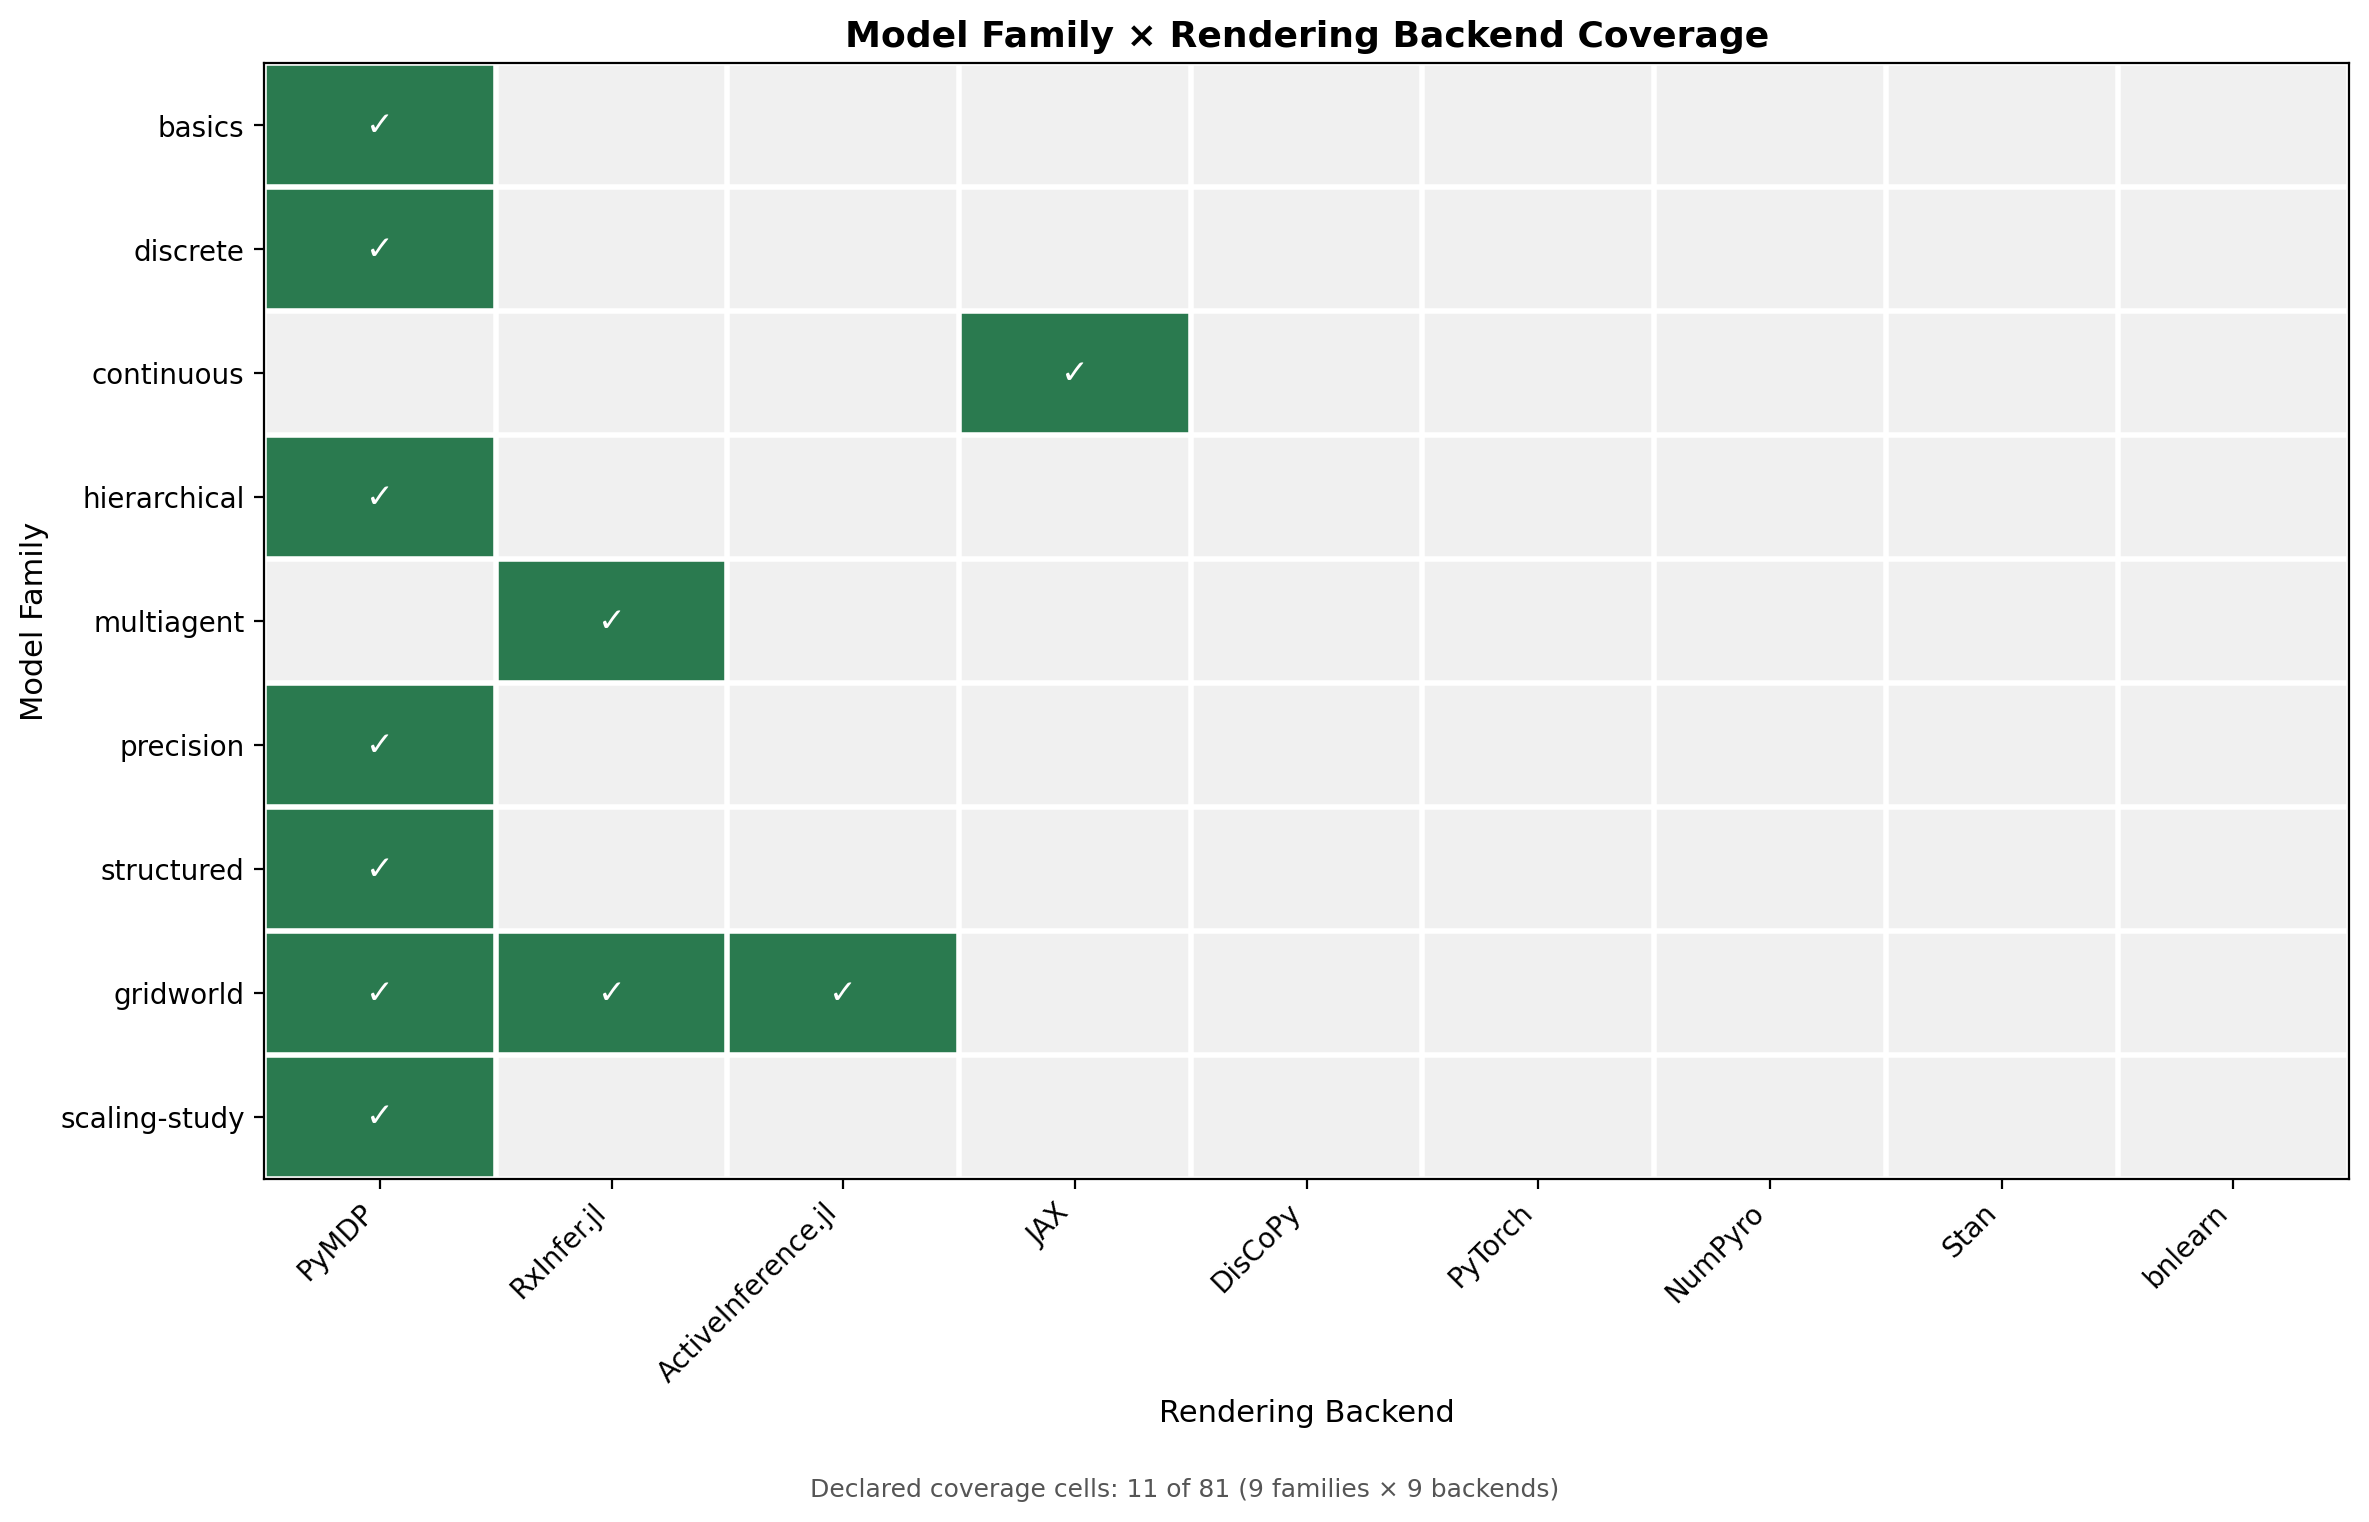
\includegraphics[width=0.85\linewidth,height=0.40\textheight,keepaspectratio,alt={Model-family coverage across simulation frameworks, generated from the GNN family registry.}]{../figures/gnn_family_framework_matrix.png}
\caption{Model-family coverage across simulation frameworks, generated
from the GNN family registry.}\label{fig:family_matrix}
\end{figure}

\end{frame}

\begin{frame}[fragile,allowframebreaks]{Model-Family Coverage}
These families are not illustrative prose: they are the inputs over
which the parser, the type checker, and the cross-framework code
generators are exercised, and they are the substrate for the reliability
gates described next.
\end{frame}

\begin{frame}[fragile,allowframebreaks]{Semantic-Fidelity and
Cross-Framework Reliability Gates}
\protect\phantomsection\label{semantic-fidelity-and-cross-framework-reliability-gates}
Two reproducible-by-command gates check that GNN's promise --- one text
model, many faithful executable renderings --- survives contact with
real backends. Both live under \texttt{scripts/} and read the same
family corpus described above, so they verify the artifacts the
manuscript actually references.

The semantic-fidelity gate,
\breaktt{scripts/run\_semantic\_fidelity\_gate.py}, checks that a model
parsed from GNN text and then re-emitted preserves its semantic content:
the state-space structure, the factor and modality declarations, and the
matrix shapes implied by a discrete Active Inference generative model
survive the round trip (Da Costa et al. 2020). It is meant to be run as
a command and to report fidelity per model, not as a static claim baked
into prose.

\end{frame}

\begin{frame}[fragile,allowframebreaks]{Semantic-Fidelity and
Cross-Framework Reliability Gates}
The cross-framework reliability gate,
\breaktt{scripts/run\_cross\_framework\_reliability.py}, takes a single
GNN model and renders it across multiple simulation backends, then
checks that the resulting executable models agree on the structure they
were generated from. The reference comparison runs on the continuous
family across JAX, NumPyro, RxInfer.jl --- three independent Active
Inference engines spanning the Python and Julia ecosystems (Heins et al.
2022). Because the same source model drives all three renderings,
disagreement between backends localizes a generator defect rather than a
modeling choice.

\end{frame}

\begin{frame}[fragile,allowframebreaks]{Semantic-Fidelity and
Cross-Framework Reliability Gates}
Both gates are stated here as commands you can run, not as asserted pass
counts. The manuscript deliberately does not quote a fixed number of
passing checks: the authoritative, current result is whatever those
scripts report when executed against the corpus, and binding a frozen
count into prose would invite exactly the drift the auto-injection
contract exists to prevent.
\end{frame}

\begin{frame}[allowframebreaks]{Repository Scale}
\protect\phantomsection\label{repository-scale}
The repository's scale is itself evidence of the surface that the gates
and pipeline cover, and it is reported in fig.~\ref{fig:repo_metrics}
directly from a scan of the working tree.

\end{frame}

\begin{frame}[allowframebreaks]{Repository Scale}
\begin{figure}
\centering
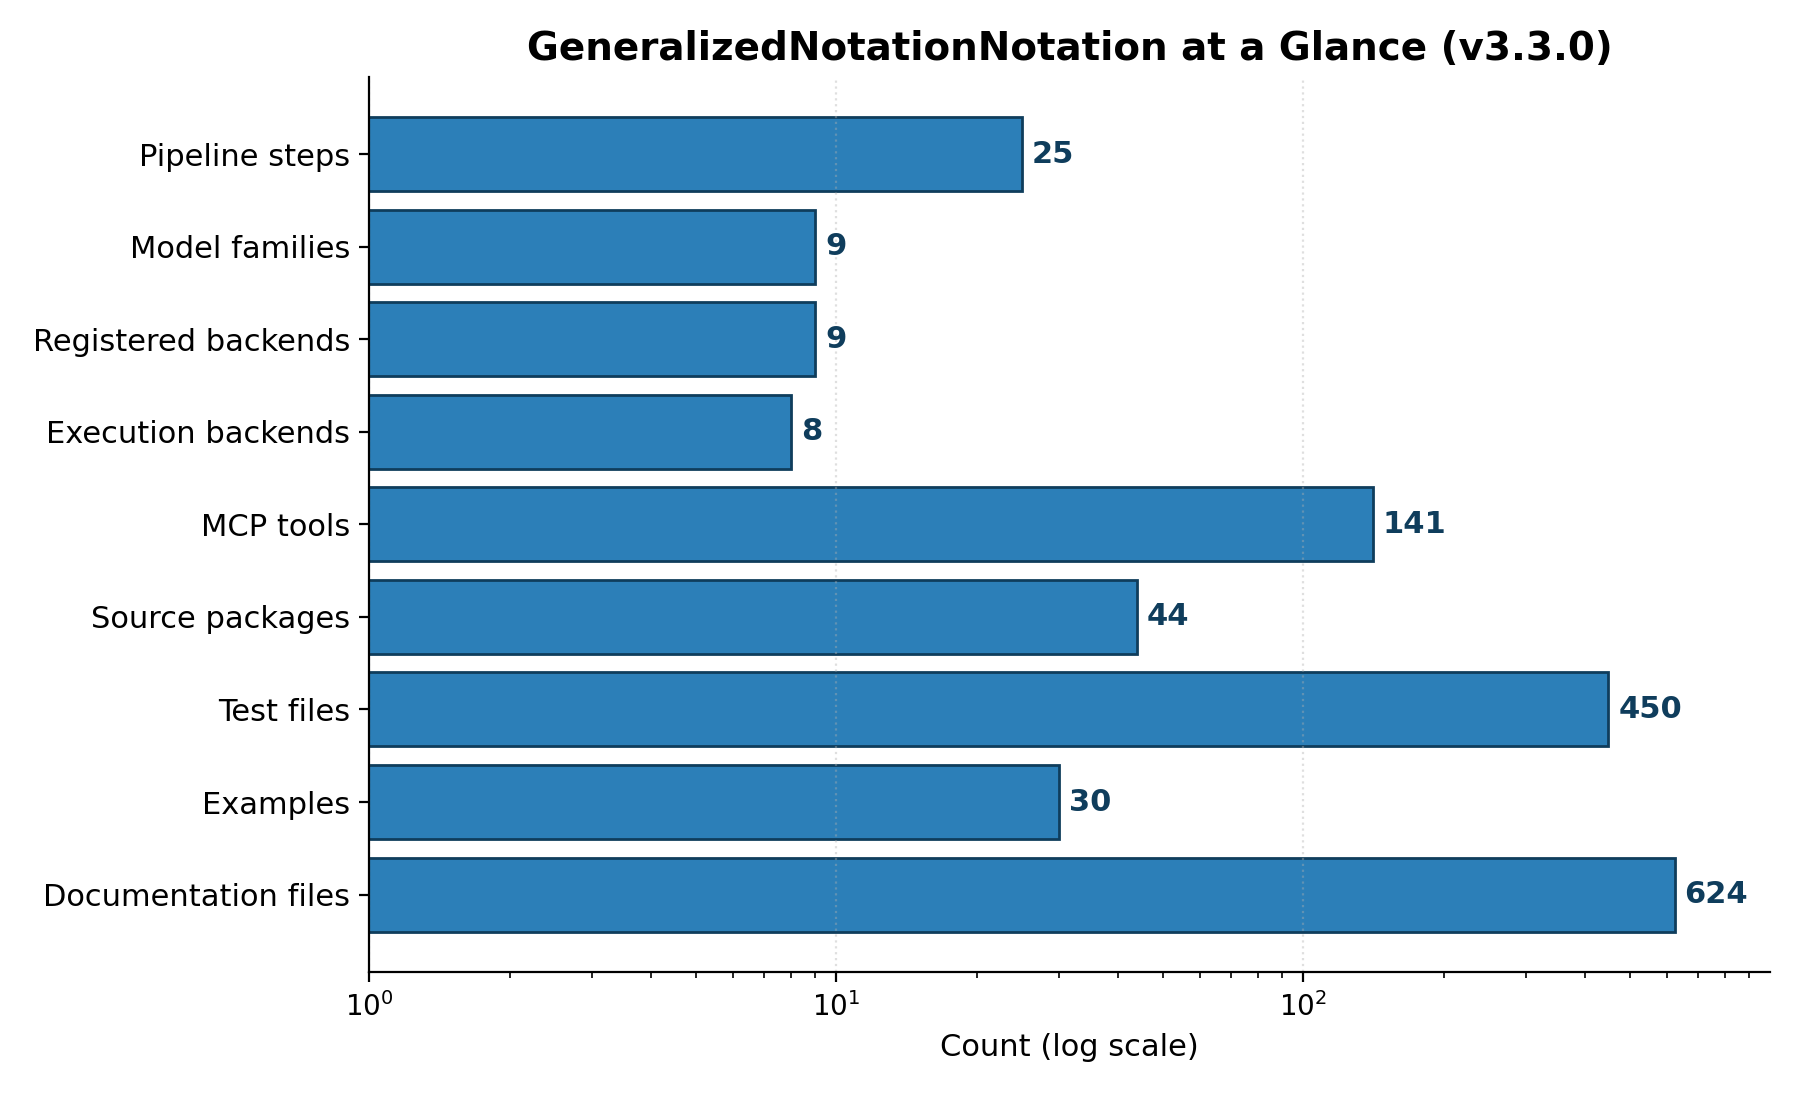
\includegraphics[width=0.8\linewidth,height=0.40\textheight,keepaspectratio,alt={Repository-scale metrics --- source packages, test files, and tool surface --- measured from the live repository.}]{../figures/gnn_repo_metrics.png}
\caption{Repository-scale metrics --- source packages, test files, and
tool surface --- measured from the live
repository.}\label{fig:repo_metrics}
\end{figure}

\end{frame}

\begin{frame}[allowframebreaks]{Repository Scale}
The test suite comprises 365 test files containing 4109 test functions,
exercising a source base of 582 Python files across 31 packages (194567
lines of source). The Model Context Protocol surface --- which exposes
GNN's capabilities to external agents and tools --- provides 141 tools
across 32 modules. The pipeline itself runs as 25 steps (0--24), and the
rendering of figures, models, and reports produced 105 figures in the
current run.
\end{frame}

\begin{frame}[fragile,allowframebreaks]{Claim Discipline}
\protect\phantomsection\label{claim-discipline}
A claim is manuscript-ready only when it is bound to a verifiable
artifact. Concretely, every claim in this manuscript must rest on one of
four support types:

\end{frame}

\begin{frame}[fragile,allowframebreaks]{Claim Discipline}
\begin{itemize}
\tightlist
\item
  A passing test or validator command --- for example the
  semantic-fidelity and cross-framework gates above, which can be re-run
  on demand.
\item
  A generated output produced by a deterministic producer, such as the
  figures rendered from the family and repository scans, or the token
  values emitted by the manuscript-variable producer that backs every
  number on this page.
\item
  A source ledger, manifest, or configuration file that fixes the value
  being claimed.
\item
  A resolved entry in \texttt{references.bib} for any
  external-literature claim (Friston 2010; Parr et al. 2022).
\end{itemize}

\end{frame}

\begin{frame}[fragile,allowframebreaks]{Claim Discipline}
The pipeline records its own evidence trail under \texttt{output/}. The
run-level summary is written to \breaktt{output/PIPELINE\_REPORT.md}, and
the per-step execution record --- including which steps ran, their
status, and their artifacts --- is captured in
\breaktt{output/00\_pipeline\_summary}. These are the artifacts a reader
should consult to confirm that the numbers substituted into this section
correspond to a real, reproducible pipeline run rather than to asserted
prose. When a value would otherwise need a literal number with no
producer behind it, the discipline is to omit the number rather than to
hard-code it.
\end{frame}

\end{document}
